% !TEX encoding = UTF-8 Unicode
\documentclass[BachelorPaper]{subfiles}
\acresetall
%Providecommands für Subfiles
    \providecommand{\citepic}[1]{(#1)}
    \providecommand{\citefig}[2]{(#1, S. #2)}
    \providecommand{\citefigm}[2]{(Modifiziert #1, S. #2)}

\begin{document}
\chapter{Material}
The following sections list the different tools used while working on the components of the BOINSO network applications.

\section{General}
\label{sec:mat_general}
This section includes tools which allow a group of developers to work on complex projects in a decentralized manner. As this project is intended to be used in an academic context and monetary resources are scarce in this field tools that are either open source or free of charge for educational programs.

\subsection{GIT-SCM}
\label{subsec:mat_git}
The \ac{git-scm} is a "[...] fast, scalable, distributed revison control system with a [...] rich command set that provides both high-level operations and full access to internals" as declared in \cite{git_scm}. It follows the same "branch -> develop -> merge" work-flow as \ac{SVN} and is freely distributed under the \ac{GPLv2}. It was originally developed by Linus Torvalds to offer Linux Kernel developers a free way to collaboratively work on a distributed code-base efficiently.

\subsection{GitHub}
\label{subsec:mat_github}
GitHub is a provider of cloud hosted \ac{git-scm} repositories. As GitHub was originally introduced by members of the open source community it still maintains a very generous relationship to open source contributors. GitHub users who publish their work to public repositories may use virtually all services bound to the GitHub infrastructure free of charge with only minimal limitations. GitHub also offers premium enterprise accounts which include a certain amount of private repositories and premium services if they are needed.

\subsection{Travis-CI}
\label{subsec:mat_travis}
Travis-CI is a web hosted continuous integration server. Continuous integration is the automated process of building and testing a project with every introduction or modification of a software component. Its goal is to assure and improve the quality of the project while alerting the development team if a change would lead to a breaking application.\\

In contrast of other continuous integration solutions like Jenkins -- an open source continuous integration server implemented in the Java programming language -- the configuration of a Travis-CI process is done by adding a simple configuration file to root of your \ac{git-scm} repository as seen in listing \ref{lst:travis.yml}.\\

\lstinputlisting[language=yaml, caption={BOINSO Travis-CI configuration file. For this file type the YAML syntax is used. The built process runs once for every Python interpreter version included in the configuration. Services like a data base connection can be included and configured prior to the built process. It is possible to include command line expressions and additional hooks which react to Travis-CI events.}, label=lst:travis.yml]{listings/.travis.yml}

\subsection{Vagrant}
\label{subsec:mat_vagrant}
Vagrant is a tool which is used to virtualize development environments. It offers a command line interface to download, start up, pause, halt and provision images of virtual machines which come configured with all the dependencies needed to develop, run and test an application. Base images can be built to closely model a production system as closely as possible being configured by a trained system administrator masking the complexity of this system from developers and designers. Depending on the base image type Vagrant users have to have access to a certain virtualization provider -- also known as hypervisor.\\

The initialization process of a Vagrant environment depends on the presence of a vagrant configuration file -- simply known as the Vagrantfile. Listing \ref{lst:Vagrantfile} depicts the Vagrantfile of the BOINSO Core Web Application.\\

\lstinputlisting[language=Ruby, caption={BOINSO Core Web Application Vagrantfile including expressions to set the virtual base box, a simple shell provisioner executing a bash script which installs variable project dependencies, and the automated port forwarding from the virtual box to the host development machine}, label=lst:Vagrantfile]{listings/Vagrantfile.rb}

Provisioning can be done by DevOps tools like Puppet or Chef or any other program used in this context. As the scope and the resources of this project are limited a simple shell provisioner was used. An example for a provisioning script can be seen in listing \ref{lst:bootstrap_prov}.\\

\lstinputlisting[language=bash, caption={Vagrant shell provisioning bash script}, label=lst:bootstrap_prov]{listings/bootstrap.sh}

\subsection{Open Source Licensing}
\label{subsec:mat_licensing}
Open source software is easy to extend and distribute as portability issues can be solved directly in the source code. Unfortunately there are numerous developers and companies which sole purpose seems to be the destruction of open source projects through the medium of patenting and licensing schemes. To protect a project and its collaborators a well established software license should be used. The \ac{FSS} provides a set of licenses and guidelines for their own licensing products and affiliated licenses. A starter guide for choosing the right free software license can be found at \cite{fss_license_guide}. Project initiator should be aware that licenses recommended by the \ac{FSS} are most likely going to be rather strict free software licenses which makes later commercial use harder in many cases. That is the reason for the BOINSO project favoring the Apache~License~2.0.

\section{BOINSO Core Web Application}
\label{sec:mat_boinso_core}
This section focuses on the tools and frameworks used to implement the core of the BOINSO Core Web Application.

\subsection{pip}
\label{subsec:mat_pip}
In a modern Python environment pip is used to manage Python modules. Pip itself is a python module which accesses the \ac{PyPI}, downloads a module and its dependencies, starts the compilation process for Python extensions and either adds the module to the global Python interpreters Python path or the path of a local virtual Python environment. Besides installing single packages on demand for console execution pip can also be used as a dependency management tool. Rather than manually managing all dependencies of a projects developers normally include a requirements.txt file to their project roots which is used by pip to install project dependencies in the right version. Listing \ref{std:requirements.txt} shows the requirements.txt file of the BOINSO Core Web Application.\\

\lstinputlisting[language=Python, caption={BOINSO Core Web Application requirements.txt file including project dependencies and their version. Version notation follows the "major.minor.patch" pattern. Omitting versioning information means that the latest available version of a module will be installed -- in this case this is not likely to cause problems as sphinx is only used to generate documentation.}, label=std:requirements.txt]{listings/requirements.txt}

\subsection{Virtualenv}
\label{subsec:mat_virtualenv}
Virtualenv is a Python command line tool to create local light weight Python environments with encapsulated tools and an isolated Python module path. Virtual environments can be activated on a per shell basis and replace the system's standard Python installation in this scope. Virtualenv is used to separate the dependencies of a distinct application from other project as different dependency versions are prone to errors when being installed to the same context.

\subsection{Django}
\label{subsec:mat_django}
Django is one of the major Python web frameworks. It is backed by a very committed developer community, easy to use, secure and scalable. Without further configuration it includes powerful management tools, database independent \ac{ORM} facilities, an intuitive template engine and an automatically generated administration interface. The project maintainers offer these tools but are very keen on making sure that all components are as modular as possible. This means that almost all components can be substituted by other established projects (e.g.: Jinja template engine instead of Django template engine or SQLAlchemy \ac{ORM} instead of Django \ac{ORM}). Besides substituting core components the Django app system also allows developers to write framework extensions which add additional functionality.\\

Django can be used to its full potential when working on data driven dynamic web applications. To give developers granular control of application functionality and to enforce a maintainable code base the framework makes extensive use of the \ac{MVC} pattern. Figure \ref{fig:MVC} shows the typical collaborative processes between the different \ac{MVC} components.

\clearpage

\begin{figure}[!htbp]
%\begin{figure}[H]
\centering
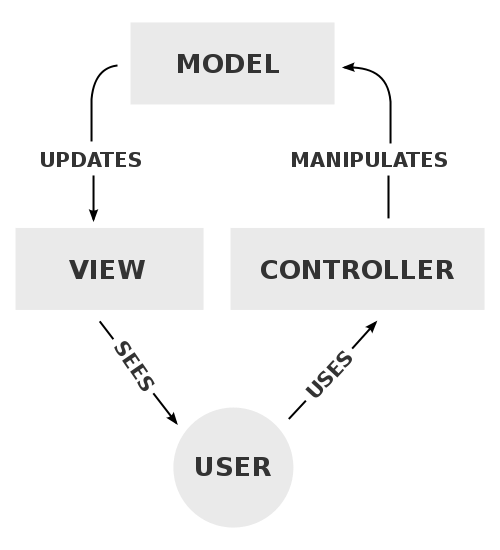
\includegraphics[width=0.5\linewidth]{PICs/BacPics/MVC-Process.png}
\caption{Typcial collaboration of MVC components \url{http://commons.wikimedia.org/wiki/File:MVC-Process.svg} Last acces: 09.05.2015}\label{fig:MVC}
\end{figure}

\lstinputlisting[language=Python, caption={BOINSO Core Web Application satellite model}, label=lst:boinso_models, firstline=22, lastline=59]{listings/models.py}

\minisec{Model}
The model is the programmatic representation of an entity. The \ac{ORM} implementation maps the different data members of the model class to a table in the databases and casts the fields to the related database vendor type implementations. An example for a simple model implementation can be seen in listing \ref{lst:boinso_models}. Besides the correct mapping to the data base the field types also allow the usage of validation chains which throw errors if input values violate input constraints.\\

\minisec{View}
The view is the layer in which data is presented to clients who can interact with it without having knowledge of the underlying logic. In classical Django applications a view is called a template and rendered to a \ac{HTML} document presented to a web browser. The BOINSO Core Web Application makes use of the Django \ac{REST} Framework where a serializer is used instead of a template. Listing \ref{lst:boinso_serializers} shows the serializer related to the satellite model shown in listing \ref{lst:boinso_models} extending a model serializer provided by the Django \ac{REST} Framework which provides resource identification and resource location by \ac{URL} fields catering to the \ac{HATEOAS} principle introduced in \cite{Fielding_2000}.\\

\lstinputlisting[language=Python, caption={BOINSO Core Web Application satellite serializer}, label=lst:boinso_serializers, firstline=89, lastline=105]{listings/serializers.py}

\minisec{Controller}
The controller reacts to signals set by the user, manipulates the state of a model and updates views. Business logic is incorporated in this component. In the Django vernacular a controller is -- to the confusion of many users -- called a view. A sample of a more complex controller is depicted in listing \ref{lst:boinso_views} where a client request containing an OAuth2 access token is used to filter for the related user object. The view establishes the connection to the serializer class and checks requests for both authentication (client is registered user) and permission (registered user has the rights to view/modify requested data).\\

\lstinputlisting[language=Python, caption={BOINSO Core Web Application UserProfileProxy}, label=lst:boinso_views, firstline=75, lastline=93]{listings/views.py}

\subsection{Nginx}
\label{subsec:mat_nginx}
Nginx is an open source reverse proxy for protocols for web and mail protocols, as well as a load balancer, cache and a web server. It is available for all major operating systems, easy to deploy and easy to configure. In the context of a deployed Django application Nginx is used to tunnel requests to the application's \ac{WSGI} server, to serve static content (images, style sheets, etc.) and to cache non dynamic content. An example for a production configuration file for a Django application using Nginx can be seen in listing \ref{lst:nginx}.\\

\lstinputlisting[caption={Nginx configuration file example. Virtual host is instructed to listen to port 8000 while limiting the maximum body size to 20 megabyte. Requests directed at the virtual host are forwarded to the local application server including the original headers. A static file request is handled by Nginx.}, label=lst:nginx]{listings/nginx.conf}

\subsection{Gunicorn}
\label{subsec:mat_gunicorn}
Gunicorn is a Python \ac{WSGI} server implemented adhering to the \ac{WSGI} definition postulated in \cite{pep_0333}. As the integrated Django development server is well suited for testing and developing but it is not suited for a production environment due to stability and security implications deployment the usage of a well established solution such as Gunicorn or uWSGI. In cases where the production environment cannot sustain aforementioned solutions (as on Windows server machines) or whenever it is simply not desired to use an additional third party solution there are also modules for the popular Apache Web Server (\ac{BSD} httpd) or the \ac{IIS}.\\

Gunicorn is normally installed as a Python module in a virtual environment. This means that there is normally no native operating system hook which starts, restarts and monitors the server processes. In a Python environment a service which can be used to keep the server alive is called supervisord. With a simple configuration file like the one in listing \ref{lst:supervisord} supervisord can handle the server life-cycle, restarting failed and zombie processes. The configuration execution itself can be handed to the operating system via the system initiator daemon (on Unix systems mostly initd, systemd or upstartd).\\

\lstinputlisting[caption={Supervisord example configuration file}, label=lst:supervisord]{listings/supervisord.conf}

\section{BOINSO MCC Web Client}
\label{sec:mat_boinso_web}
This section focuses on the tools and frameworks used to implement the client side web client for the BOINSO application.

\subsection{AngularJS}
\label{subsec:mat_angular}
AngularJS is a client side JavaScript \ac{MVC} framework for constructing single page applications. A single page application -- written using \ac{HTML}, \acp{CSS} and JavaScript -- offers rich client experience incorporating a modular and testable design. In contrast to classic web applications where every navigation results in a new request and the download of all web resources a single page application loads all the static content on the first request loading dynamic asynchronously on demand.\\

A concept heavily used in AngularJS is the Inversion of Control (or dependency injection) paradigm. Functionality shared by different objects is encapsulated in services which are listed as object dependencies. Injected dependencies (or instances thereof) become part of the object's state and can be called as if they were original members. In test situations those services can be easily exchanged by mock objects improving component isolation.\\

To make templates in AngularJS semantically more expressive it is possible to implement custom directives. This process loosely resembles the working draft for custom elements (also known as web components) as stipulated in \cite{w3c_custom_elements_2014}. In many cases this fact can be used to distribute compact application modules as directives which are easy to use and configure.

\subsection{Stylus}
\label{subsec:mat_stylus}
Stylus is a \ac{CSS} precompiler language which is used to write styling information in a more efficient and readable way. \ac{CCS} precompilers offer programming language features like arithmetic expressions, variable declarations, function declarations and selector nesting which are not part of the official \ac{CSS}3 implementation. With the addition of stylus modules mundane and repetitive tasks like adding vendor prefixes, or working with basic typographic definitions can be solved automatically.

\subsection{Node Package Manager}
\label{subsec:mat_npm}
The \ac{npm} is used to manage NodeJS packages. Many JavaScript projects are already deployed to the node package index and can be used as a managed dependency. For using \ac{npm} as a local dependency management and build tool a package configuration file as seen in listing \ref{lst:package.json} can be added to the project's root directory.\\

\lstinputlisting[language=JavaScript, caption={BOINSO MCC Web Client package configuration. Used to include project specific meta data, deployment and development dependencies, and script definitions.}, label=lst:package.json]{listings/package.json}

\subsection{Bower}
\label{subsec:mat_bower}
Bower is a package manager similar to \ac{npm}. Traditionally it is used in situation in which pure front-end components are installed without the need of a deep dependency tree. Bower can be configured at a per project basis with a configuration file as displayed in listing \ref{lst:bower.json}.\\

\lstinputlisting[language=JavaScript, caption={BOINSO MCC Web Client bower configuration. Used to include project specific meta data in case the deployment to the bower package index is a project goal as well as front-end dependencies.}, label=lst:bower.json]{listings/bower.json}

\subsection{Bootstrap}
\label{subsec:mat_bootstrap}
Bootstrap is is a \ac{HTML}, \ac{CSS}, and JavaScript framework for developing responsive, mobile first web applications. It is distributed and maintained by Twitter, available under the \ac{MIT} license and easy to adjust in pure \ac{CSS}, Sass or less (both being \ac{CSS} precompiler languages). It offers an easy to use grid system and a tool set of isolated responsive components as well as commonly used utility classes.

\section{Boinso GPredict Bridge}
\label{sec:mat_boinso_bridge}
This section focuses on the tools used in the conception of the piece of middleware that connects \acp{GCC} using GPredict to their related \acp{MCC}.

\subsection{GPredict}
\label{subsec:mat_gpredict}
GPredict is an application which allows users to track orbiters communicating elevation and azimuth values to the rotator control daemon (a \ac{HamLib} utility) while also transferring Doppler shift parameters -- alternation of radio frequencies due to high velocity movement of orbiting objects -- to the rig control daemon (a \ac{HamLib} utility controlling the radio). Independent from the way in which the client is finally implemented many parts of the aforementioned projects should be incorporated into the project because they have an extensive community and decrease the projects complexity immensely.\\

The BOINSO project relies on a modified version of GPredict which automatically switches between a list of orbiters which is stored in a module definition. Those orbiters are represented by their file representations in the GPredict data directories and might additionally include transponder definitions which can be used to fine tune the Doppler shift calculations.

\end{document}
